\section{Introduction}
\label{sec:introduction}

\begin{figure*}[t!]
\centering
  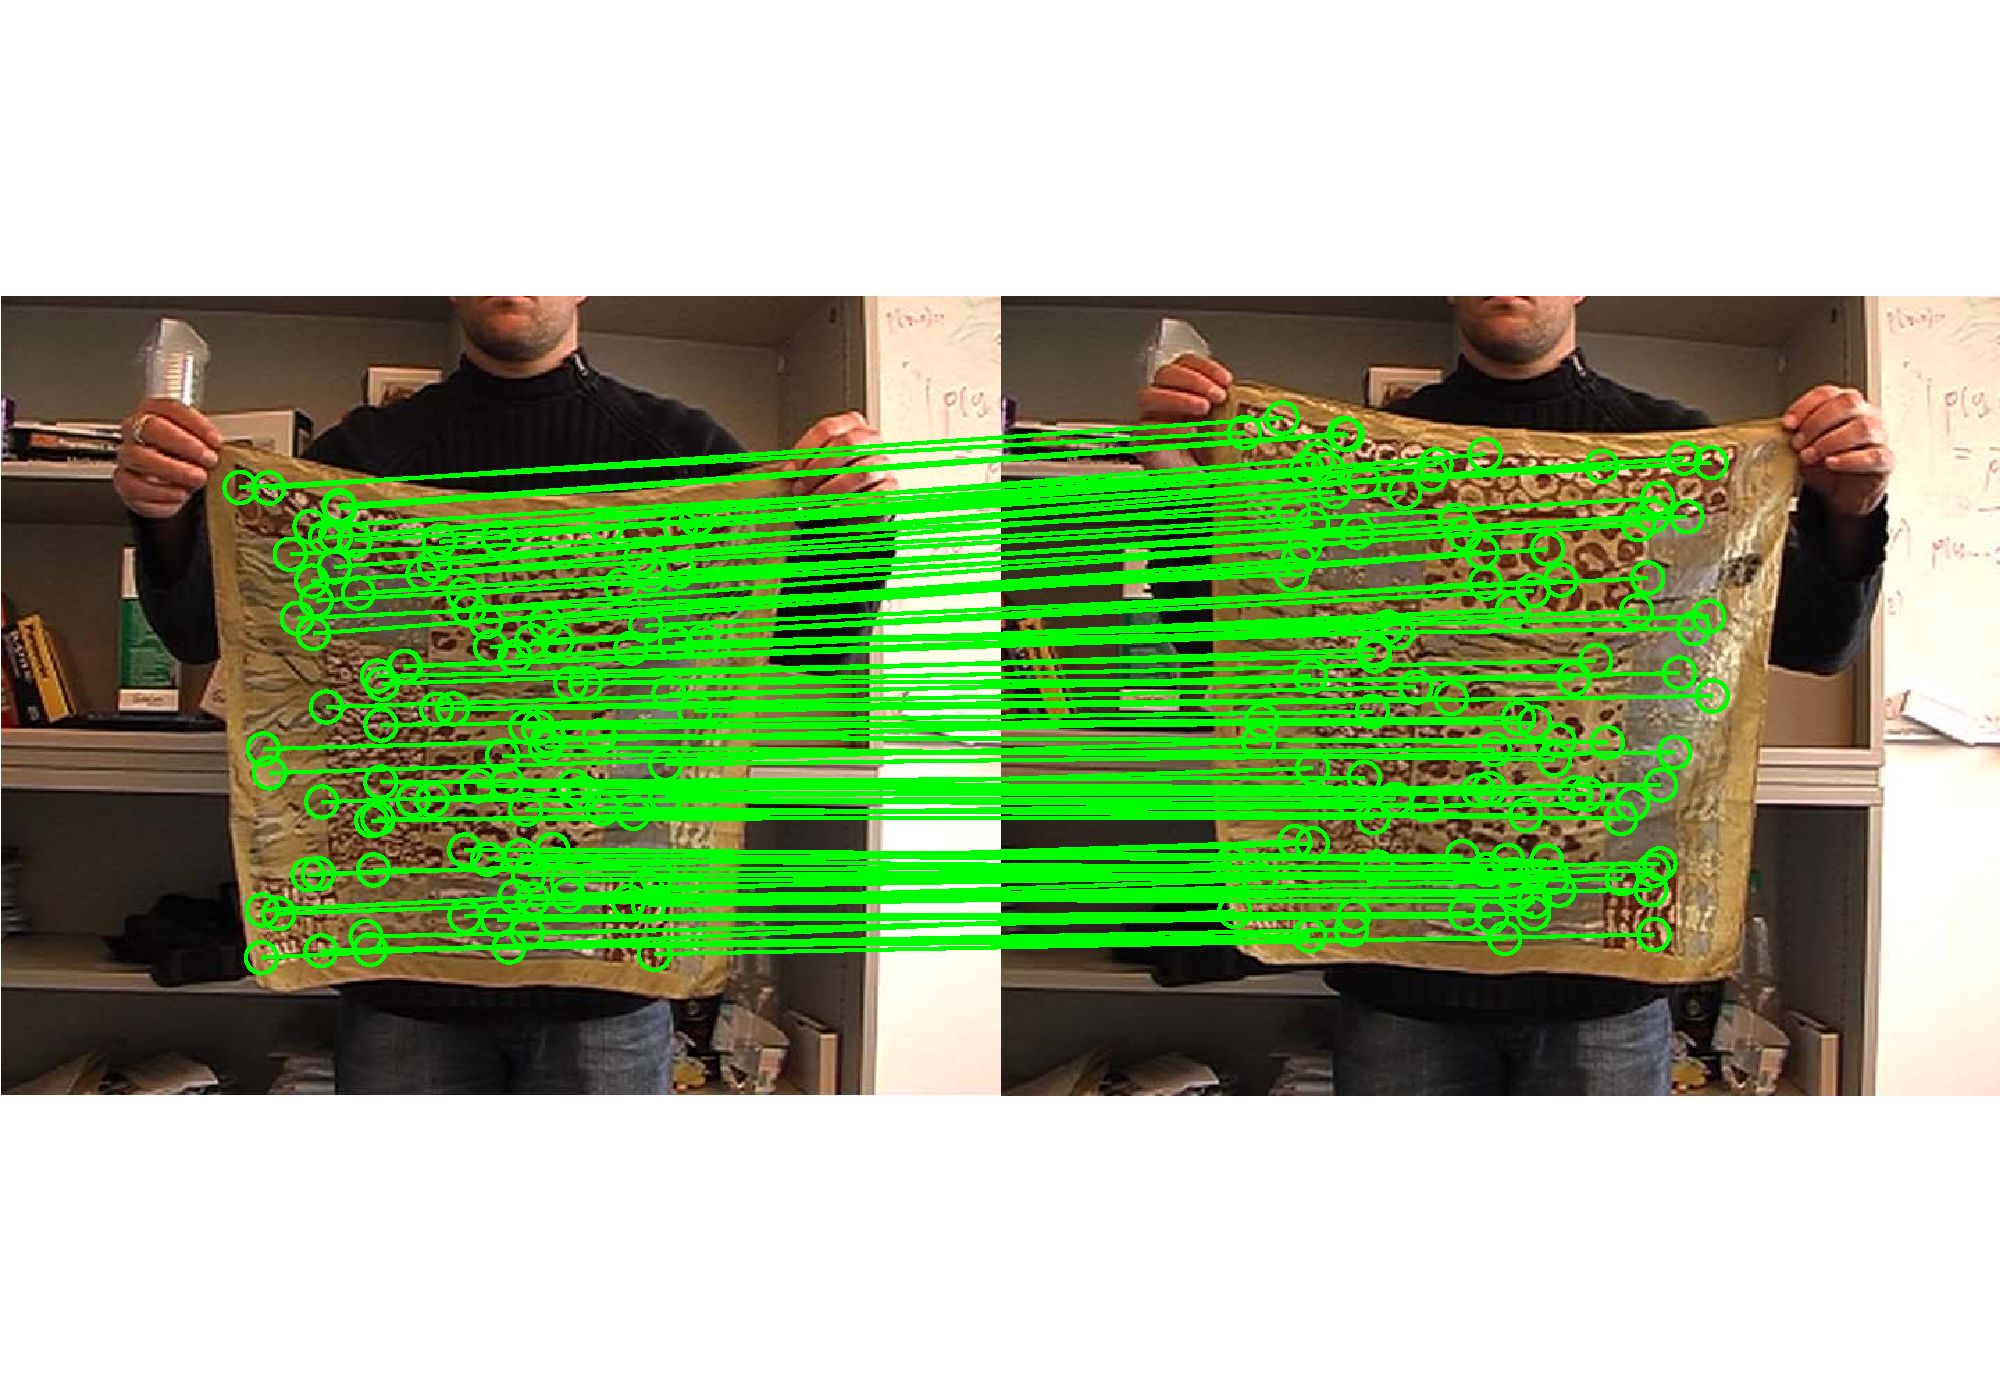
\includegraphics[width=0.98\linewidth]{figures/teaser2.pdf}
  \caption{Correspondences between datasets determined by SuperMatching, using feature points created simply by uniform sampling rigid scans on the left, and SIFT feature points on a deformable surface on the right. For clarity, only some representative matches are shown.}
\label{fig:teaser}
\end{figure*}

Building correspondences between two sets of features belonging to a pair of 2D images or 3D shapes
is a fundamental problem in many computer graphics, geometry processing, and computer vision tasks.
It arises in applications such as
registration of partial or entire 3D shapes~\cite{Besl92,Gelfand05,Aiger08,li08,Chang09,Zeng10,vanKaick11,Chang11},
shape retrieval from databases~\cite{Bronstein11},
shape matching~\cite{Berg05,Brown07,Lorenzo08,Tevs09,Ovsjanikov10,Tevs11,SahilliogluY11,Windheuser11},
shape reconstruction~\cite{Brown07,Pekelny08,Wand09,Chang11},
and automatic shape understanding~\cite{Huttenlocher90,Lipman09,Sun10,Kim11} .

Determining correspondences is typically done in three steps~\cite{Johnson99,Lowe04,Sun09,Toler10,Leutenegger11}:
(i) computing high-quality descriptors which serve to distinguish points from one another,
(ii) choosing certain salient points with unusual feature descriptors, for matching,
and (iii) determining the most suitable matching between the two sets of points.
The former two problems have attracted considerable attention; their importance is clear.
However, even supposing ideal feature descriptors and selectors that capture the most important and distinctive information about the neighborhood of each salient point,
state-of-the-art algorithms  still find it challenging to determine the best matching~\cite{vanKaick11}:  real input data is noisy, and data may only be approximately in correspondence.
The problem is further complicated by the presence of symmetric and congruent regions.
Various feature matching algorithms have been devised to be robust in the presence of such issues. RANSAC-like algorithms~\cite{Tevs09,Tevs11} minimize the effects of outliers,
while generalized multidimensional scaling~\cite{Bronstein11} and
heat kernel maps~\cite{Ovsjanikov10}  consider the manifold in which the points are embedded. M{\"o}bius transformations~\cite{Lipman09,Kim11} also provide a powerful approach.
However, these previous algorithms generally do not treat the matching step as an independent problem, even if matching is not tightly coupled with feature description and selection.
This paper focuses on the feature matching problem as a problem in its own right.

Matching may be done pointwise (single points to single points), or using tuples of points:
e.g.\ point pairs, separated by a fixed distance, to other point pairs,
triples of points forming a triangle to other triples of points, and so on.
As pointed out by~\cite{Conte04}, matching single features leads to
a linear assignment problem, but if multiple features are matched simultaneously,
a quadratic or higher-order assignment problem results.
Matching two feature sets by considering similarities of \emph{single} features from each set can easily fail in the presence of ambiguities such as repeated elements,
or similar local appearance.
Quadratic and higher-order assignment matches groups of features,
enforcing other constraints such as consistency of distances between the points in each tuple being matched.
Doing so helps to reject many false matches, greatly improving the matching output.
Feature similarity and satisfaction of constraints may in general be expressed in terms of an affinity tensor relating pairs of point tuples.

As a particular example of \emph{quadratic} assignment, Leordanu and Hebert~\cite{Leordeanu05} consider pairs of feature descriptors,
and use \emph{distances} between pairs of features from each set to reduce the number of incorrect correspondences.
Such pairwise distance constraints are particularly helpful in cases when the features themselves have low discriminative ability.
The idea has been widely adopted in 3D shape matching algorithms~\cite{Tevs09,Ovsjanikov10,Tevs11,Kim11,SahilliogluY11,Windheuser11}.

Higher-order assignment  includes yet more complex constraints between features.
For example, third-order potential functions, used in~\cite{Duchenne09,Duchenne2011,Zeng10,Chertok10,Aiping10},
quantify the affinity between two point triples by measuring the similarity of the angles of the triangles formed by such triples.
However, this angular similarity value only considers the \emph{total} difference in corresponding angles, and does not change with reordering of elements in the tuple.
When similarity is expressed in this way, the affinity tensor becomes a \emph{supersymmetric} tensor~\cite{Kofidis02}.

Our \emph{SuperMatching} algorithm also formulates higher-order matching problems using a supersymmetric affinity tensor. It can accurately match a moderate number
of features (several hundreds) using triples or larger tuples of features.
%It goes beyond previous approaches in that:
The contributions of this paper include:
\begin{itemize}
\item We show how to define a compact higher-order supersymmetric affinity tensor to express geometrically consistent constraints between feature tuples.

\item Complete computation of the full affinity tensor is computationally infeasible. We efficiently estimate it using a sampling strategy which takes advantage of supersymmetry. This avoids sampling repetitive items, it allows the tensor to be stored compactly, and also improves the matching accuracy by avoiding imbalances in sampling.

\item We make full use of the compactness of the affinity tensor to deduce a power iteration method which efficiently solves the matching problem.
\end{itemize}

Our experiments using both synthetic and real captured data sets show that SuperMatching is more accurate and robust than prior methods,
yet has similar computational cost.
Importantly, it is a general matching approach, independent of choice of 2D or 3D feature descriptors.
%feature point selection method, and constraints placed on tuples.
